$\indent$ Fracture process in atomic scale is a complex process controlled by the local structure of atoms, stress applied, and forces between atoms and the strength of atomic bonds. Given the large amount of simulation data generated from LAMMPS (Large-scale Atomic/Molecular Massively Parallel Simulator) \cite{PAMD}, which is a molecular dynamics program from Sandia National Laboratories, we are going to develop a machine learning algorithm to predict the fracturing process.

\begin{itemize}

\item \textbf{Graph Representation}


In order to be able to predict the atomic scale fracture nucleation and propagation in silica-based glasses, we must first find an appropriate mathematical graph representation. 
\begin{itemize}
    \item \textbf{Basic Graph Representation}
    \\
    \\
    The most basic way to define a graph is naive. In one sample, we have a total number of $n$ atoms. An atom, either silicon or oxygen, is defined as a vertex $v_i$, where $0 \leq i \leq n-1$ and a set of such vertices is $\mathbf{\textbf{V}} = \{v_0,v_1,...v_{n-1}\}$. An edge, $e_i$ is defined as a chemical bond between two atoms. A set of such edges is $\mathbf{E} = \{e_0,e_1,...e_{n-1}\}$. As uni-axial stress is applied to the material, edges could break and form between any two vertices, where state 1 means an edge is broken and state 0 means an edge exists.
    %Therefore, a set of active edges, defined as $\mathbf{E_a}$, includes all the edges that have broke or formed at least once, meaning they have changed their state, either from 1 to 0 or from 0 to 1 at one point. Similarly, $\mathbf{V_a}$ is defined as a set of active atoms.
    As a result, the graph $\mathbf{\textbf{G}}$ is thus defined as a discrete set of vertices $\mathbf{V}$ connected by a set of edges $\mathbf{E}$. We can denote it as $\ \mathbf{G} = (\mathbf{V},\mathbf{E})$, where the size of the graph is $\ |\mathbf{V}| = n $.
    \\
    \\
    A simplified example of our constructed graph could result like this:
    \bigskip
    \\
    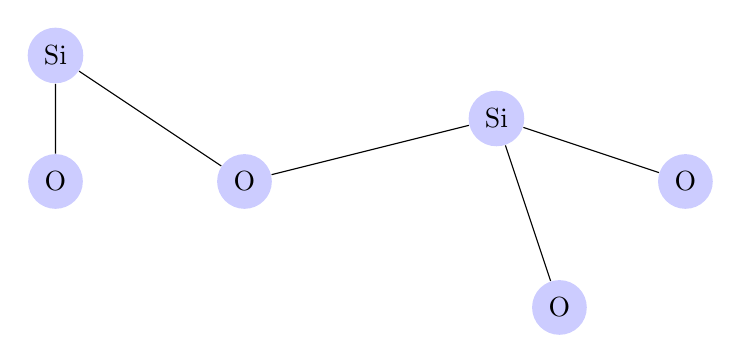
\begin{tikzpicture}
      [scale=.8,auto=left,every node/.style={circle,fill=blue!20}]
      \node (n6) at (1,10) {Si};
      \node (n4) at (4,8)  {O};
      \node (n5) at (8,9)  {Si};
      \node (n1) at (11,8) {O};
      \node (n2) at (9,6)  {O};
      \node (n7) at (1,8)  {O};
    
      \foreach \from/\to in {n6/n4,n4/n5,n5/n1,n2/n5,n6/n7}
        \draw (\from) -- (\to);
    
    \end{tikzpicture}
    
\item \textbf{Reduced Graph Representation} 

A possible reduced graph representation would be to consider only silicon atoms as nodes and each of their bonds as edges. This would reduce computational complexity. We would take into account the data regarding $Q_n$ to construct this graph.
    
\end{itemize}


\item \textbf{The Ground Truth}

In this project, we will use supervised learning technique. To train a supervised machine learning model, examples of input-output pairs are needed. Each of these pairs have the input and the desired output for the corresponding input. So, the ground truth, denoted as $y_i$ for atom $i$, is the desired output we want our model to predict. To be more specific, it is defined as whether or not an atom is part of a fracture at a certain time step. If $y_i$ is in state 0, it means it is not part of a fracture, and $y_i$ is in state 1, it means it is part of a fracture. So $\mathbf{y}$ is a vector of length $n$, where $n$ is the total number of atoms at each time step. And $y_i\in\{0,1\}$ for $i\in\{1,2,3,...,n\}$. This can be different as to which problem we are trying to solve. In the goals section, we state that our goal is split into two problems. As a result, the ground truth can be a little different in each setting.

\begin{itemize}
    \item \textbf{In nucleation}
    
    Nucleation event is the creation of void in the material. As stress is applied uni-axially, bonds break and form among atoms. Correspondingly, some atoms have growing void among themselves and others are squished into more dense regions. And fracture nucleates alongside the void occurrence. 
    \begin{figure}
    \centering
    \noindent
    \includegraphics[width=0.7]{volcolor.PNG}
    \caption{Crack propagation}
    \label{crack_Fig}
\end{figure}
    As a result, we define the ground truth using a local density measure, which is the Voronoi cell volume $v_i$, around a certain atom $i$. Previously, flexibility volume has been used as an indicator for prediction of stress driven shearing in atomic structures of glasses \cite{NatCom}. It is a volume measure because the data is a 3D graph and we are measuring the volume of the polyhedron centered by the atom. So, if $v_i$ exceeds a certain threshold, then atom $i$ is defined as part of a nucleation event, which also means $y_i=1$. In this project, we set the threshold to be 3 standard deviation from the mean value, $\mu_v$, at the current time step.
    \textbf{1. Could insert a figure here demonstrating 3D Voronoi volume}
    \textbf{2. Could insert 3 figures demonstrating why we choose 3sd as our threshold}
    \[
    nuc_v = \frac{(v_i - \mu_v)}{\sigma_v}
    \]
    And then the ground truth can be defined as:
    \[
    y_i = \begin{cases}
      0 & \text{if nuc_v$_i \le 1 $}\\
      1 & \text{if nuc_v$_i \ge 1 $}\\
    \end{cases} 
    \]  
    \item \textbf{In propagation}
    
    Contrary to a fracture nucleation event, the propagation is where the fracture grows along the existing fracture. Some atoms are part of the fracture but they are surrounded by other atoms, which results in a small Voronoi volume. To compensate for these false negatives, we will look at local neighborhoods of the atoms considered as part of the fracture. As a result, we use the K-nearest Neighbors (KNN) algorithm to identify positive atoms, meaning atoms with $y_i=1$. \textbf{Insert a figure showing an atom and its k-nearest neighbors}.
    
\end{itemize}


\item \textbf{Feature Description}
\bigskip

To use ML algorithms, we want to examine features of our system such as centrality, volume, and structure.

\begin{itemize}
    \item \textbf{Centrality:} In graph theory, centrality is used to identify the most important vertices. An example could be a specific silicon atom that is at the center of where a fracture nucleates. Identifying the vertices with the highest centrality will allow us to predict fracture nucleation.
    
    \bigskip
    
    More specifically, the vertex with the highest centrality degree would be surrounded by the most active bonds. Bonds that are not active do not necessarily contribute to the nucleation of a fracture \cite{valera2018machine}.
    
    \begin{itemize}
        \item \textbf{Degree Centrality Measures:} We will use Degree Centrality Measures. This measure indicates how connected a vertex is by counting the direct links each vertex has to other vertices. Our network will be simplified to active bonds, therefore, the more links a vertex has to other vertices, the more connected that vertex is to active bonds. This will allow us to better understand where a fracture propagates from. 
    \end{itemize}
    
    \bigskip
    
    Additionally, we want to use the local properties of the atoms as features. The local features are available from the molecular dynamics post processing done. 
    This includes the size of a fracture and the speed of propagation. We aim to use eigenvector centrality measure which will lend a deeper understand as to what the connections a vertex with a high degree centrality has to the entire network. This is because eigenvector centrality measures the influence that a vertex has on an entire graph. Therefore, we can examine vertices that are associated with fractures and analyze what their effect is on the overall behavior of the glass.
    
    \begin{itemize}
        \item \textbf{Eigenvector Centrality Measures } Eigenvector Centrality Measures indicates how much influence a specific vertex has on the entire network. For example, consider a vertex that has a high degree centrality, but does not necessarily affect the network. Therefore, it must have a low eigenvector centrality and does not contribute to a fracture that significantly damages the network. For this reason, we want to consider which vertices have a high eigenvector centrality measure in connection with degree measures. Doing so will lead us to a deeper understanding of where fractures nucleate and what the propagation of  these fractures looks like.
    \end{itemize}
\item \textbf{$Nuc_v$ and $Nuc_d$:} Within our data set are the features $nuc_v$ and $nuc_d$ which are measures of volume and displacement. By color coding our system, we are able to examine how volume gives a measure of local density. As atoms move away from one another, the local density increases. This can be visualized in our graph. Therefore, volume can help our model understand which atoms are closely associated with fracture nucleation by examining how and where volume increases.

\item\textbf{$Q_n$:} An additional feature in our data is $Q_n$ which allows us to quantify the structure. When considering the number of oxygen atoms bonded to a single silicon atom, $Q_n$ indicates the number of oxygen that are bridging one another. This is defined as an Si-O-Si group where the oxygen is bridging. This gives rise to the connectivity of our system.

\item\textbf{Stress Tensor:} Stress tensor defines the state of stress at a specific point of a material. We aim to examine the stress tensor at specific atoms which is provided to us in the data. By looking at this feature, we can see if there exists a range of stress tensor values that lead to a fracture. Doing so will provide more insight as to wear a fracture might occur as a result of the degree of stress that is applied to the glass \cite{mWilson_continuum_stress} \cite{elastic_fracture}.

\item\textbf{Charges:} We will take the charge of each atom in account to examine what effect each charge has in forming a fracture. The real values in our data represent the effects of quantum fluctuations from shifts of electron clouds. Charge plays a significant role in the bond between atoms. It is important to note that high charges indicate strong forces between atoms. Therefore, there is more activity. We want to investigate whether high charges are directly associated to active sets. 
\end{itemize}

 We aim to predict a final fracture surface and nucleation points given an initial state. After the model has been created, we will begin feature analysis to determine which characteristics of our system play a significant role in the accuracy of our predictions.
\\

\item \textbf{Machine Learning Methods}
\bigskip
\\
The culminating purpose of this project is to produce a surrogate model of the molecular dynamic simulations using supervised machine learning techniques. We propose to address our two goals listed above with two methods, respectively. First, use an ensemble of random forest to predict the nucleation based on local structures. Second, predict the Vonoroi volume of an atom, and use the prediction to interpret whether or not an atom is part of the fracture. Therefore this section of the methods will address our proposed ML architecture from start to finish.


\begin{itemize}
\bigskip
\item \textbf{Method for Classifying whether or not a vertex is part of a fracture in the nucleation setting}
\bigskip
\\
%Random forest. Boosting, bagging. 
For the purpose of determining whether or not a vertex is associated with a fracture, we will implement ensemble based ML methods. The goal of ensemble methods is to combine predictions made by several features into one single learned estimator. With our feature selection being possibly quite large, we will find ensemble methods being the best option to predict fracture labels. 
\bigskip
\\
Core ensemble methods include boosting and bagging. A "bagged" random forest method is generated by creating a tree from the features randomly drawn with replacement. Since our representation is graph like these trees make sense logically. 
\bigskip
\\
Our algorithm will look like this:
\\
1. Take training set T with N features, with L models.
\\
2. For model $L _{1}$ let the number of input points $n_{1}$ $<$ $N$ for each $L_{n}$.
\\
3. For model $L_{n}$, create a training set by choosing $d_{l}$ features from T with replacement and train the model.
\bigskip
\\
Adaboost however is a boosting method which learns from previous mistakes made during training. By learning previous mistakes the model can increase the weights of incorrectly predicted points from the training data. 
\bigskip
\\
Our algorithm will look like this:
\\
1. Initialize weights of the features. 
\\
2. Train a decision tree.
\\
3. Find the error weighed rate and calculate the tree's weight in the overall ensemble. 
\\
4. For every feature wrongly predicted, update the weight. 
\\
5. Repeat until complete. 
\item \textbf{Method for Predicting the Voronoi Cell Volume Dynamically}
\bigskip
\\
%RNN, 
Due to the dynamical structure of our graph changing over each time step we will be implementing a Long short-term memory(LSTM) neural network to predict $v_i$ of the atoms at each time step. The input will be a time series of Voronoi cell volume for all the atoms at time step $t$, which is a vector of length $n$.

\begin{figure}
    \centering
    \noindent
\includegraphics[width=0.4\textwidth]{picture/frac_prop1.PNG}\hspace{0.2\textwidth}%
\includegraphics[width=0.4\textwidth]{picture/frac_prop2.PNG}\\[2em]
\includegraphics[width=0.4\textwidth]{picture/frac_prop3.PNG}\hspace{0.2\textwidth}%
\includegraphics[width=0.4\textwidth]{picture/frac_prop4.PNG}\par
    \caption{Crack propagation}
    \label{rnn}
\end{figure}







After we have obtained a time series of predicted $v_i$, we compare the prediction with the threshold, which is 3 standard deviation from the mean, to determine whether a certain atom is part of a fracture or not. Similar with what is defined before:
    \[
    \hat{y_i} = \begin{cases}
      0 & \text{if nuc_v$_i \le 1 $}\\
      1 & \text{if nuc_v$_i \ge 1 $}\\
    \end{cases} 
    \]  

\bigskip
\bigskip
\\

\item \textbf{Machine Learning from start to finish}
\bigskip
\\
The proposed architecture is as follows
\bigskip
\\
\tikzstyle{decision} = [diamond, draw, fill=blue!20, 
    text width=4.5em, text badly centered, node distance=3cm, inner sep=0pt]
\tikzstyle{block} = [rectangle, draw, fill=blue!20, 
    text width=5em, text centered, rounded corners, minimum height=4em]
\tikzstyle{line} = [draw, -latex']
\tikzstyle{cloud} = [draw, ellipse,fill=red!20, node distance=3cm,
    minimum height=2em]
    
\begin{tikzpicture}[node distance = 2cm, auto]
    % Place nodes
    \node [block] (init) {MD Simulation Data};
    \node [block, below of=init] (features) {Extracted Features};
    \node [block, below of=features] (training) {Training Set};
    \node [block, left of=training, node distance=3cm] (test) {Test Set};
    \node [block, right of=training, node distance=3cm] (validate) {Validation Set};
    \node [decision, below of = training] (RF) {Random Forest};
    \node [decision, below  of = test] (rnn) {LSTM};
    \node [cloud, below of = RF] (out) {Surrogate Model};
    %\node [cloud, below of= RF, node distance=3cm] (pof) {RF Output};
    %\node [cloud, below of= rnn, node distance=3cm] (rnnout) {RNN Output};

    % Draw edges
    \path [line] (init) -- (features);
    \path [line] (features) -- (validate);
    \path [line] (features) -- (training);
    \path [line] (features) -- (test);
    \path [line] (training) -- (RF);
    \path [line] (training) -- (rnn);
    \path [line] (rnn) -- (out);
    \path [line] (RF) -- (out);
    \path [line] (validate) |- node [near end] {} (out);
\end{tikzpicture}

\bigskip
    1. First we analyze and determine features from the MD data.
    \\
    2. Extract the features and prepare data for training. 
    \newline
    3. Split the dataset into three sets: training, validation, and test.
    \newline
    4a. Train the training set using RF to predict which atoms are part of a fracture.
    \newline
    4b. Train the data using LSTM to predict vertices displacement.
    \newline
    5. Validate surrogate model using validation set. 
    \newline
    6. Feature analysis. Fine tune features which are deemed most important. 
    \newline
    7. Finalize surrogate model on test set. 




\end{itemize}


\end{itemize}